\documentclass[12pt,b5paper]{ltjsarticle}

%\usepackage[margin=15truemm, top=5truemm, bottom=5truemm]{geometry}
%\usepackage[margin=10truemm,left=15truemm]{geometry}
\usepackage[margin=10truemm]{geometry}

\usepackage{amsmath,amssymb}
%\pagestyle{headings}
\pagestyle{empty}

%\usepackage{listings,url}

% 記号変更
%\renewcommand{\theenumi}{(\arabic{enumi})}
\renewcommand{\labelenumi}{(\arabic{enumi})}


%\usepackage{graphicx}

\usepackage{tikz} % draw graphics : TikZ ist kein Zeichenprogramm
%\usetikzlibrary{arrows.meta} % 矢印のカスタマイズ

%\usepackage{wrapfig}
%\usepackage{bm} % ベクトルの矢印

%\usepackage{luatexja-ruby} % ルビを振る

%% 核Ker 像Im Hom を定義
\newcommand{\Ker}{\mathop{\mathrm{Ker}}\nolimits}
\newcommand{\Img}{\mathop{\mathrm{Img}}\nolimits}
%\newcommand{\Hom}{\mathop{\mathrm{Hom}}\nolimits}

%\DeclareMathOperator{\Rot}{rot}
%\DeclareMathOperator{\Div}{div}
%\DeclareMathOperator{\Grad}{grad}
%\DeclareMathOperator{\arcsinh}{arcsinh}
%\DeclareMathOperator{\arccosh}{arccosh}
%\DeclareMathOperator{\arctanh}{arctanh}

\usepackage{url} % URLの記述

%\usepackage{listings}
%
%\lstset{
%%プログラム言語(複数の言語に対応，C,C++も可)
%  language = Python,
%%  language = Lisp,
%%  language = C,
%  %背景色と透過度
%  %backgroundcolor={\color[gray]{.90}},
%  %枠外に行った時の自動改行
%  breaklines = true,
%  %自動改行後のインデント量(デフォルトでは20[pt])
%  breakindent = 10pt,
%  %標準の書体
%%  basicstyle = \ttfamily\scriptsize,
%  basicstyle = \ttfamily,
%  %コメントの書体
%%  commentstyle = {\itshape \color[cmyk]{1,0.4,1,0}},
%  %関数名等の色の設定
%  classoffset = 0,
%  %キーワード(int, ifなど)の書体
%%  keywordstyle = {\bfseries \color[cmyk]{0,1,0,0}},
%  %表示する文字の書体
%  %stringstyle = {\ttfamily \color[rgb]{0,0,1}},
%  %枠 "t"は上に線を記載, "T"は上に二重線を記載
%  %他オプション：leftline，topline，bottomline，lines，single，shadowbox
%  frame = TBrl,
%  %frameまでの間隔(行番号とプログラムの間)
%  framesep = 5pt,
%  %行番号の位置
%  numbers = left,
%  %行番号の間隔
%  stepnumber = 1,
%  %行番号の書体
%%  numberstyle = \tiny,
%  %タブの大きさ
%  tabsize = 4,
%  %キャプションの場所("tb"ならば上下両方に記載)
%  captionpos = t
%}

%\usepackage{cancel}
%\usepackage{bussproofs}
%\usepackage{proof}

\begin{document}


\begin{equation}
 \int_{-\infty}^{\infty} \frac{e^{-ix}}{(1+x^{2})^{2}} \mathrm{d}x
  \qquad (x\in \mathbb{R})
\end{equation}


\hrulefill

$\exp{z}$は$\mathbb{C}$上正則関数

\begin{equation}
 \exp{\left( z \right)} = \sum_{n=0}^{\infty} \frac{z^{n}}{n!}
\end{equation}

$1/(1+z^{2})^{2}$は$z=\pm i$に極を持つ。
\begin{equation}
 \frac{1}{(1+z^{2})^{2}}
  = \frac{1}{(z+i)^{2}} \cdot \frac{1}{(z-i)^{2}}
  = \frac{1}{(z-i)^{2} + 4i(z-i) -4} \cdot \frac{1}{(z-i)^{2}}
\end{equation}

$e^{-iz}$を$z=i$を中心にTaylar展開する。
\begin{equation}
 e^{-iz}
  = e \sum_{n=0}^{\infty} \frac{(-i)^{n}}{n!}(z-i)^{n}
\end{equation}

これにより次の Laurent展開が得られる。
\begin{equation}
\frac{e^{-iz}}{(1+x^{2})^{2}}
 = 
 \frac{e}{(z+i)^{2}} (z-i)^{-2}
 +
 \frac{-ie}{(z+i)^{2}} (z-i)^{-1}
 +
 e \sum_{n=0}^{\infty} \frac{(-i)^{n+2}}{(n+2)!}(z-i)^{n}
\end{equation}


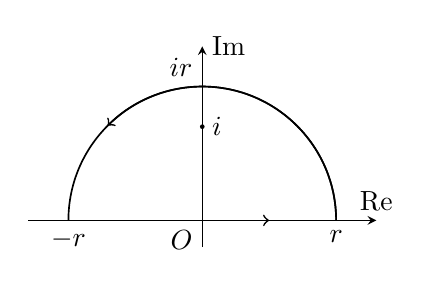
\begin{tikzpicture}[scale=1.7]
 \coordinate (XS) at (-1.3,0); % x軸最小
 \coordinate (XL) at (1.3,0); % x軸最大
 \coordinate (YS) at (0,-0.2); % y軸最小
 \coordinate (YL) at (0,1.3); % y軸最大

% \draw[semithick,->,>=stealth] (XS) -- (XL) node[above]{Re}; % x軸
 \draw[->,>=stealth] (XS) -- (XL) node[above]{Re}; % x軸
 \draw[->,>=stealth] (YS) -- (YL) node[right]{Im}; % y軸
 \draw (0, 0) node[below left] {$O$}; % 原点

 \draw[semithick] (1,0) arc (0:180:1); % 円弧
 \draw[semithick, ->] (1,0) arc (0:135:1); % 円弧

 \draw[semithick] (-1,0) -- (1,0); % 線分
 \draw[semithick, ->] (-1,0) -- (0.5,0); % 線分



 \draw (1, 0) node[below] {$r$}; % 数値
 \draw (-1, 0) node[below] {$-r$}; % 数値
 \draw (0, 1) node[above left] {$ir$}; % 数値

 \fill (0, 0.7) circle (0.5pt); % ポイントプロット
 \draw (0, 0.7) node[right] {$i$}; % 数値
\end{tikzpicture}

$r\in\mathbb{R}$
\begin{equation}
 C_{1} = \{ t\in\mathbb{R} \mid -r\leq t \leq r \}
 ,\quad
 C_{2} = \{ re^{i\theta} \mid 0 \leq \theta \leq \pi \}
\end{equation}


\begin{equation}
 \left|
 \int_{C_{2}}
  \frac{e^{-iz}}{(1+z^{2})^{2}} \mathrm{d}z
       \right|
 =
 \left|
 \int_{C_{2}}
  \frac{e^{-i(\cos{\mathrm{Re}z}+i\sin{\mathrm{Im}z})}}{(1+z^{2})^{2}} \mathrm{d}z
       \right|
 \leq
 \left\lvert \frac{e^{-iz}}{(1+z^{2})^{2}} \right| \cdot
 \left\lvert C_{2} \right\rvert
 \leq 
\end{equation}


\hrulefill









\end{document}
